\documentclass{article}
\usepackage[utf8]{inputenc}
\usepackage[a4paper, top=2cm, bottom=2cm, left=2.5cm, right=2.5cm]{geometry}
\usepackage{hyperref}
\usepackage{graphicx}
\usepackage{float} 
\usepackage{subfigure}
\usepackage{amssymb}
\usepackage{fancyhdr}
\usepackage{algorithm}
\usepackage{algpseudocode}

\usepackage[sorting=none]{biblatex}
\addbibresource{reference.bib}

\title{SOEN 6011 Project Documentation \\
\large https://github.com/hbcbs110/SOEN6011-project}
\author{Shuo Gao \\ 40203484 \\ Concordia University}
\date{Summer 2022}

\makeatletter
\newenvironment{breakablealgorithm}
  {% \begin{breakablealgorithm}
   \begin{center}
     \refstepcounter{algorithm}% New algorithm
     \hrule height.8pt depth0pt \kern2pt% \@fs@pre for \@fs@ruled
     \renewcommand{\caption}[2][\relax]{% Make a new \caption
       {\raggedright\textbf{\ALG@name~\thealgorithm} ##2\par}%
       \ifx\relax##1\relax % #1 is \relax
         \addcontentsline{loa}{algorithm}{\protect\numberline{\thealgorithm}##2}%
       \else % #1 is not \relax
         \addcontentsline{loa}{algorithm}{\protect\numberline{\thealgorithm}##1}%
       \fi
       \kern2pt\hrule\kern2pt
     }
  }{% \end{breakablealgorithm}
     \kern2pt\hrule\relax% \@fs@post for \@fs@ruled
   \end{center}
  }
\makeatother

\begin{document}

\pagestyle{fancy}
\fancyhf{}
\maketitle
\pagenumbering{roman}
\tableofcontents
\newpage
\pagenumbering{arabic}

\fancyfoot[C]{\thepage}
\addcontentsline{toc}{section}{Problem 1}
\rhead{Problem 1}
\section{Description}
Function used: tan(x)
The function tan(x), which is called tangent function, is one of the trigonometric functions (also called circular functions), which are real functions relating an angle of a right-angled triangle to the ratio of two side length. The trigonometric functions are widely used in all sciences and technologies. For an acute angle $\theta$ in a right triangle, the tangent function can be defined as: $tan(\theta)=\frac{opposit}{adjacent}$.\cite{enwiki:1101002187} Here is a graph of tan(x) below in Figure 1:

\begin{figure}[H]
\centering
\subfigure[circular functions]{
\label{Fig.sub.1}
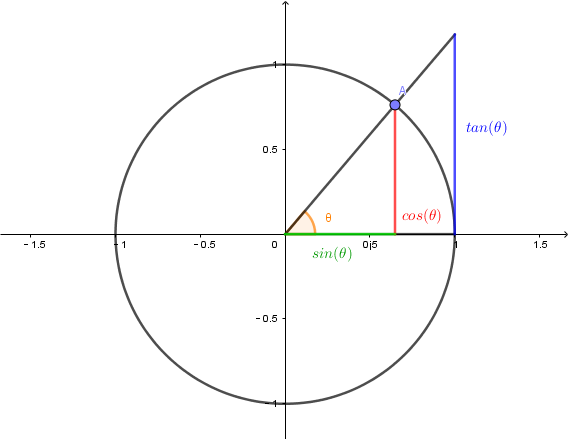
\includegraphics[width=0.45\textwidth]{unitcicletan.png}}
\subfigure[graph of tan(x)]{
\label{Fig.sub.2}
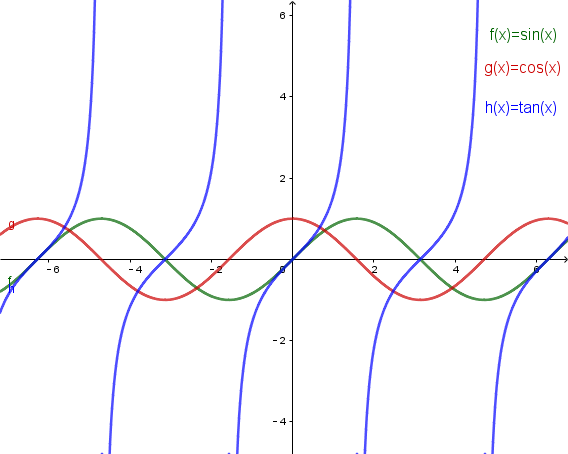
\includegraphics[width=0.45\textwidth]{tanfuncgraph.png}}
\caption{Graph of tangent function tan(x)}
\label{Fig.main}
\end{figure}

\subsection{Domain and co-domain}
\begin{enumerate}
    \item \textbf{Domain}: $\{x\in\mathbb{R}|x\ne k\pi+\frac{\pi}{2}, k\in\mathbb{Z}\}$
    \item \textbf{Co-domain}: $(-\infty, +\infty)$ All real number $\mathbb{R}$
\end{enumerate}

\subsection{Characteristics}
\begin{enumerate}
    \item $tan(x)=\frac{sin(x)}{cos(x)}$
    \item period: $\pi$
    \item vertical asymptotes: $x=\frac{\pi}{2}+k\pi, k\in\mathbb{Z}$
    \item $tan(a\pm b)=\frac{tan(a)\pm tan(b)}{1\mp tan(a)tan(b)}$
    \item $tan(-x)=-tan(x)$
\end{enumerate}

\section{Context of use model}
The model below is based on the guideline in IEEE Guide for Information Technology System Definition Concept of Operation (ConOps) Document.\cite{1998ieee}
\begin{enumerate}
    \item User: A user who is going to calculate the value of tan(x) with the input x using a calculator.
    \item Task: Calculate the output of tan(x) given the input x and who the result on the screen to the user.
    \item Environment:
    \begin{itemize}
        \item Technical environment: Power supply of the calculator. Runtime environment.
        \item Non-technical environment: Location of the user while using the calculator.
    \end{itemize}
\end{enumerate}


\newpage
\addcontentsline{toc}{section}{Problem 2}
\rhead{Problem 2}
\section{Requirement}

\subsection{Introduction}
Requirements below are written based on the the styles and guidelines given in the ISO/IEC/IEEE 29148 Standard, section 5.2.4 to 5.2.8.\cite{8559686}

\subsection{Requirements Set}
\begin{enumerate}
    \item Requirement \arabic{enumi}
    \begin{itemize}
        \item Identification: FR1
        \item Version Number: 1.0
        \item Owner: Shuo Gao
        \item Stakeholder Priority: High
        \item Risk: Low
        \item Description: The user shall make sure that he/she inputs a real number, or a valid double number. The real number may contains numbers from 0 to 9, period ".", letter e, and plus or minus sign "+" and "-".
        \item Rationale: The function tan(x) only supports real numbers as input. To avoid error of calculating
        \item Difficulty: Easy
        \item Type: Functional Requirement
    \end{itemize}
    \item Requirement \arabic{enumi}
    \begin{itemize}
        \item Identification: FR2
        \item Version Number: 1.0
        \item Owner: Shuo Gao
        \item Stakeholder Priority: High
        \item Risk: Low
        \item Description: The input of the tan(x) fanction should be radians, not degrees.
        \item Rationale: For the convenience of calculating and implementation of the algorithm, the argument of a trigonometric function is defined as the radians of angle. There for the function tan(x) takes radians as input.
        \item Difficulty: Easy
        \item Type: Functional Requirement
    \end{itemize}
    \item Requirement \arabic{enumi}
    \begin{itemize}
        \item Identification: FR3
        \item Version Number: 1.0
        \item Owner: Shuo Gao
        \item Stakeholder Priority: High
        \item Risk: Low
        \item Description: Each time the tan(x) function handles only one input and generates one output.
        \item Rationale: For the convenience of calculating, the program processes one input at a time.
        \item Difficulty: Easy
        \item Type: Functional Requirement
    \end{itemize}
    \item Requirement \arabic{enumi}
    \begin{itemize}
        \item Identification: FR4
        \item Version Number: 1.0
        \item Owner: Shuo Gao
        \item Stakeholder Priority: High
        \item Risk: Low
        \item Description: The function tan(x) should output a correct result, at least 8 to 10 digits are precise.
        \item Rationale: As a calculator the output should be correct and the precision should be in a practical range.
        \item Difficulty: Easy
        \item Type: Functional Requirement
    \end{itemize}
    \item Requirement \arabic{enumi}
    \begin{itemize}
        \item Identification: NFR1
        \item Version Number: 1.0
        \item Owner: Shuo Gao
        \item Stakeholder Priority: High
        \item Risk: Low
        \item Description: The function should return the result shortly.
        \item Rationale: Calculator needs good performance.
        \item Difficulty: Easy
        \item Type: Non-Functional Requirement
    \end{itemize}
    \item Requirement \arabic{enumi}
    \begin{itemize}
        \item Identification: NFR2
        \item Version Number: 1.0
        \item Owner: Shuo Gao
        \item Stakeholder Priority: High
        \item Risk: Low
        \item Description: The program must run in the environment where JRE(Java Runtime Environment) is installed.
        \item Rationale: The program is based on Java programming language and it requires JRE to run. Thus JRE have to be installed in the environment.
        \item Difficulty: Easy
        \item Type: Non-Functional Requirement
    \end{itemize}
    \item Requirement \arabic{enumi}
    \begin{itemize}
        \item Identification: NFR3
        \item Version Number: 1.0
        \item Owner: Shuo Gao
        \item Stakeholder Priority: High
        \item Risk: Low
        \item Description: The calculator should not crash when there is an exception during input or calculating.
        \item Rationale: Reliability.
        \item Difficulty: Easy
        \item Type: Non-Functional Requirement
    \end{itemize}
\end{enumerate}

\subsection{Assumptions}
\begin{enumerate}
    \item The input number x should be a real number in radian.
    \item The input should not be a string or an expression.
    \item If the input is not a valid number, an exception will be thrown and ask the user to input again.
    \item The output of the function will be a real number in $(-\infty, +\infty)$.
\end{enumerate}


\newpage
\addcontentsline{toc}{section}{Problem 3}
\rhead{Problem 3}
\section{Algorithm}

\subsection{Mind Map}
\begin{figure}[H]
\centering
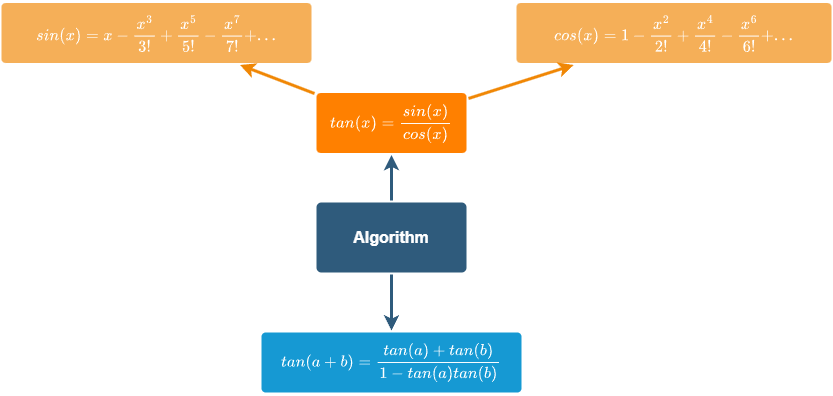
\includegraphics[width=0.6\textwidth]{mindmap.png}
\caption{Mind map}
\label{Fig.main2}
\end{figure}

\subsection{Algorithm 1}
By definition, tan(x) can be calculated with formula $tan(x)=\frac{sin(x)}{cos(x)}$. So we can calculate sin(x) and cos(x) first then tan(x). They can be calculated using Taylor series shown below\cite{enwiki:1101002187}:
$$sin(x)=\sum_{n=0}^{\infty}\frac{(-1)^{n}x^{2n+1}}{(2n+1)!}=x-\frac{x^{3}}{3!}+\frac{x^{5}}{5!}-\frac{x^{7}}{7!}+...$$
$$cos(x)=\sum_{n=0}^{\infty}\frac{(-1)^{n}x^{2n}}{(2n)!}=1-\frac{x^{2}}{2!}+\frac{x^{4}}{4!}-\frac{x^{6}}{6!}+...$$
\begin{breakablealgorithm}
\caption{}
\begin{algorithmic}
\Require $x \in \mathbb{R}$
\Ensure $y = tan(x)$
\State $x \gets input$
\State $y \gets sin(x)/cos(x)$
\newline
\Function{sin}{$x$}
    \State {$sign \gets f \gets 1$} \Comment{Sign and factorial factor of each term}
    \State {$a \gets x$} \Comment{Term of Taylor series without factor}
    \State {$s \gets 0$} \Comment{Result of sin(x)}
    \For{$i \gets 1$ to $100$} \Comment{Process Taylor series}
        \State {$s \gets s+sign\times a/f$}
        \State {$a \gets a \times x \times x$}
        \State {$sign \gets -sign$}
        \State {$f \gets f\times (2 \times i + 2) \times (2 \times i +3)$}
    \EndFor
    \State \Return {$s$}
\EndFunction
\newline
\Function{cos}{$x$}
    \State {$sign \gets f \gets 1$} \Comment{Sign and factorial factor of each term}
    \State {$a \gets 1$} \Comment{Term of Taylor series without factor}
    \State {$c \gets 0$} \Comment{Result of cos(x)}
    \For{$i \gets 1$ to $100$} \Comment{Process Taylor series}
        \State {$c \gets c+sign\times a/f$}
        \State {$a \gets a \times x \times x$}
        \State {$sign \gets -sign$}
        \State {$f \gets f\times (2 \times i + 1) \times (2 \times i +2)$}
    \EndFor
    \State \Return {$c$}
\EndFunction
\end{algorithmic}
\end{breakablealgorithm}

\subsection{Algorithm 2}
The function tan(x) has a characteristic below:
$$tan(a + b)=\frac{tan(a) + tan(b)}{1 - tan(a)tan(b)}$$
Based on this characteristic, we can iteratively add small numbers into the angle until it reaches x. Assuming x is greater than zero, if not let $x=-x$ using the characteristic that $tan(-x)=-tan(x)$. Then the tan(x) can be calculated as below:
$$x_0=0, x_{i+1}=x_i+\Delta_i, x_n=x$$$$tan(x_{i+1})=\frac{tan(x_i) + tan(\Delta_i)}{1 - tan(x_i)tan(\Delta_i)}$$

The $\Delta_i$ and $tan(\Delta_i)$ are pre-defined constant values and $\Delta_{i+1} \leq \Delta_i < x$ for all $i$. All we need to do is iteratively calculate the value until $x_i=x_n=x$.
\newline
\begin{breakablealgorithm}
\caption{}
\begin{algorithmic}
\Require $x \in \mathbb{R}$
\Ensure $y = tan(x)$
\State $x \gets input$
\State $x_0 = 0$
\State $y \gets 0$
\State $i \gets 0$
\While{$x_0<x$ and $i<length(\Delta)$} \Comment{Iterate}
    \State $y \gets (y+tan(\Delta_i))/(1-y \times tan(\Delta_i))$
    \State $x_0 \gets x_0+\Delta_i$ \Comment{Accumulate $x_i$}
    \State $i \gets i+1$
\EndWhile
\end{algorithmic}
\end{breakablealgorithm}

\subsection{Technical Reasons of Selecting Each Algorithm}
\subsubsection{Algorithm 1}
\begin{itemize}
    \item \textbf{Advantages}: Result is more precise.
    \item \textbf{Disadvantages}: Longer than Algorithm 2. Factorial may overflow if too many terms in Taylor series are used.
\end{itemize}
\subsubsection{Algorithm 2}
\begin{itemize}
    \item \textbf{Advantages}: As an iterative algorithm it is easier to implement. Will not overflow during calculating.
    \item \textbf{Disadvantages}: Not as precise as Algorithm 1. The $\Delta_i$ and $tan(\Delta_i)$ need to be defined in advance.
\end{itemize}


\newpage
\addcontentsline{toc}{section}{Problem 4}
\rhead{Problem 4}
\section{Implementation and Debugging}
\subsection{Implementation}
The function is implemented from scrach in Java. No built-in library like Math provided by Java is used. The source code implementing Algorithm 1 and Algorithm 2 are Function.java and Function2.java. They are compiled into Function.jar and Function2.jar. The user interface is textual and error handling is supported. Below are some screenshots of the interface and error messages.
\begin{figure}[H]
\centering
\subfigure[Output of Function.java]{
\label{Fig.sub.s1}
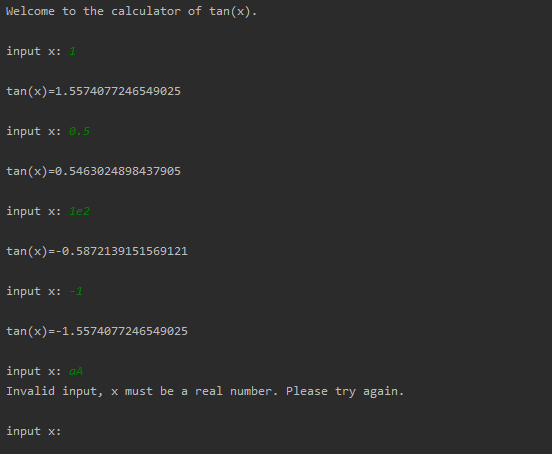
\includegraphics[width=0.55\textwidth]{runshot1.png}}
\subfigure[Output of Function2.java]{
\label{Fig.sub.s2}
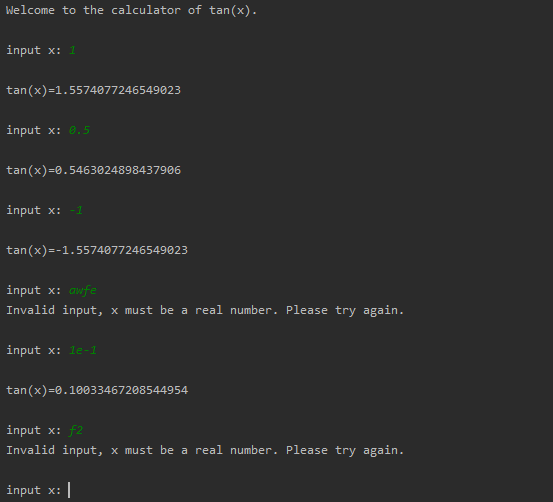
\includegraphics[width=0.55\textwidth]{runshot2.png}}
\caption{Results of the program}
\label{Fig.main3}
\end{figure}

\newpage
\subsection{Debugging}
In order to debug efficiently, the built-in debugger of the IDE IntelliJ IDEA is used. The debugger is a powerful tool. It allows users to monitor and interfere with the code and quickly catch the bugs in their code. As a built-in tool, it works well with IDE itself. Users can easily access it and debug with it during coding. The IDE provided multiple configurations of it and each process such as resume, step over and step into is easy to access. To monitor a variable, users can easily type name of the variable or just use the editor of IDE to select it. Breakpoint can be added by clicking the left side of the editor and can also be modified during debugging. The figure \ref{Fig.debug} shows the screen shot of the debugger.
\begin{itemize}
    \item \textbf{Advantages}: As a built-in debugger it is integrated well with the IDE. It has GUI and easy to process. It provides real time feed back.
    \item \textbf{Disadvantages}: Sometimes it is slow when monitoring too many variables or variables which take large space. It is not so powerful when monitoring multi-thread or multi-process program.
\end{itemize}
\begin{figure}[H]
\centering
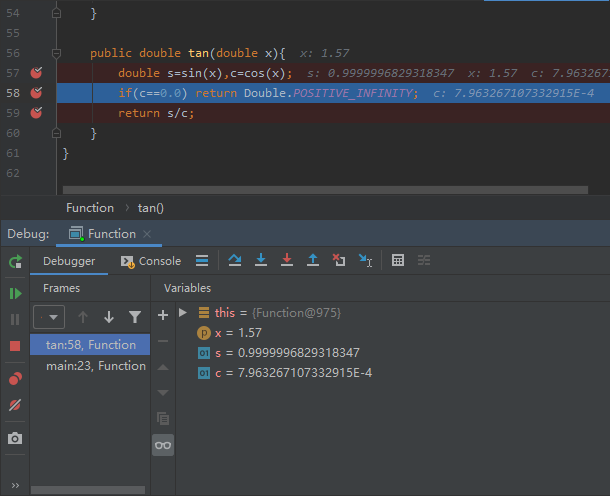
\includegraphics[width=0.6\textwidth]{debugger.png}
\caption{Debugger in Intellij IDEA}
\label{Fig.debug}
\end{figure}

\newpage
\subsection{Quality}
\subsubsection{Source code}
Each algorithm of the code only contains one source code file and it does not require outer data to run. It only requires JRE (Java Runtime Environment) to run. During runtime, the function iteratively calculates each term of a series and does not store the previous data. Therefore, the code is space-efficient and portable. The source code is short and well organized with functions. Each functions take charge of one calculating task and can be easily debugged. Thus the code is maintainable.

\subsubsection{Program}
After debugging and testing the source code, the program is confirmed correct under a certain error limit. The program might crush when user inputs a string which is not a valid real number or a double number, or is a real number that causes divided by zero error, and this situation can be avoided by error handling. When there is an invalid input, an error message is thrown telling the user to try again. This makes the program robust. To get the correct answer efficiently, the algorithms are well designed. In both algorithm 1 and algorithm 2, the loops will only run hundreds of times in total. The result can be calculated almost instantly with well precision. Users can quickly get the correct answer which shows the program time-efficient and usable.\newline

\subsubsection{Pragmatic Quality}
In order to check and maintain the pragmatic quality of the Java source code, the tool \textbf{Checkstyle} is used. It is a tool that helps programmers write Java code that adheres to a coding standard. It can check many aspects of the source code, find class design problems, method design problems, and also be able to check layout and formatting issues. In IDE IntelliJ IDEA Checkstyle is installed as a plugin and used within the IDE shown in figure \ref{Fig.checkstyle}. It checks the source code following the specific rule standard.
\begin{itemize}
    \item \textbf{Advantages}: Can find violations of code conventions. The rules can be customized.
    \item \textbf{Disadvantages}: It only check coding conventions but can't find bugs. Some of the information may not be necessary.
\end{itemize}
\begin{figure}[H]
\centering
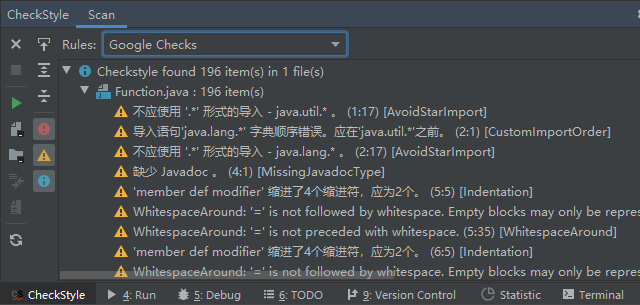
\includegraphics[width=0.8\textwidth]{checkstyleshot.png}
\caption{Checkstyle}
\label{Fig.checkstyle}
\end{figure}



\newpage
\addcontentsline{toc}{section}{Problem 5}
\rhead{Problem 5}
\section{Unit Test}
The unit test is performed with JUnit. Here are the test cases below.
\begin{enumerate}
    \item Test Case \arabic{enumi}
    \begin{itemize}
        \item input: 0.0
        \item output of Algorithm 1: 0.0
        \item output of Algorithm 2: 0.0
        \item expected output: 0.0
        \item result: Pass
    \end{itemize}
    \item Test Case \arabic{enumi}
    \begin{itemize}
        \item input: 1.0
        \item output of Algorithm 1: 1.5574077246549025
        \item output of Algorithm 2: 1.5574077246549023
        \item expected output: 1.55740772465490223
        \item result: Pass
    \end{itemize}
    \item Test Case \arabic{enumi}
    \begin{itemize}
        \item input: -1.0
        \item output of Algorithm 1: -1.5574077246549025
        \item output of Algorithm 2: -1.5574077246549023
        \item expected output: -1.55740772465490223
        \item result: Pass
    \end{itemize}
    \item Test Case \arabic{enumi}
    \begin{itemize}
        \item input: 0.5
        \item output of Algorithm 1: 0.5463024898437905
        \item output of Algorithm 2: 0.5463024898437906
        \item expected output: 0.5463024898437905
        \item result: Pass
    \end{itemize}
    \item Test Case \arabic{enumi}
    \begin{itemize}
        \item input: 1.5
        \item output of Algorithm 1: 14.101419947171722
        \item output of Algorithm 2: 14.10141994717149
        \item expected output: 14.101419947171719
        \item result: Pass
    \end{itemize}
    \item Test Case \arabic{enumi}
    \begin{itemize}
        \item input: 1.57
        \item output of Algorithm 1: 1255.76559150
        \item output of Algorithm 2: 1255.76559150
        \item expected output: 1255.76559150
        \item result: Pass
    \end{itemize}
    \item Test Case \arabic{enumi}
    \begin{itemize}
        \item input: -1.5
        \item output of Algorithm 1: -14.101419947171722
        \item output of Algorithm 2: -14.10141994717149
        \item expected output: -14.101419947171719
        \item result: Pass
    \end{itemize}
    \item Test Case \arabic{enumi}
    \begin{itemize}
        \item input: 1e2
        \item output of Algorithm 1: -0.5872139151569121
        \item output of Algorithm 2: -0.5872139151569177
        \item expected output: -0.5872139151569291
        \item result: Pass
    \end{itemize}
    \item Test Case \arabic{enumi}
    \begin{itemize}
        \item input: 3.1415926535897932384626
        \item output of Algorithm 1: 0.0
        \item output of Algorithm 2: 0.0
        \item expected output: 0.0
        \item result: Pass
    \end{itemize}
    \item Test Case \arabic{enumi}
    \begin{itemize}
        \item input: 2.5e4
        \item output of Algorithm 1: -1.0180399498523853
        \item output of Algorithm 2: -1.0180399498567576
        \item expected output: -1.0180399498575736
        \item result: Pass
    \end{itemize}
    \item Test Case \arabic{enumi}
    \begin{itemize}
        \item input: 1e6
        \item output of Algorithm 1: -0.37362445390517723
        \item output of Algorithm 2: -0.3736244538993233
        \item expected output: -0.3736244539875990
        \item result: Pass
    \end{itemize}
\end{enumerate}


\newpage
\renewcommand{\headrulewidth}{0pt}
\fancyhf{}
\addcontentsline{toc}{section}{References}
\printbibliography


\end{document}
